\documentclass[12pt]{article}
\usepackage{amsmath} % AMS Math Package
\usepackage{bm}
\usepackage{amsthm} % Theorem Formatting
\usepackage{amssymb}    % Math symbols such as \mathbb
\usepackage{graphicx} % Allows for eps images
\usepackage[dvips,letterpaper,margin=1in,bottom=0.7in]{geometry}
\usepackage{tensor}
\usepackage{amsmath}
\usepackage{siunitx}
\usepackage{physics}
\usepackage{amsmath, amssymb, graphics, setspace}
\usepackage{listings}
\usepackage{color}

\definecolor{dkgreen}{rgb}{0,0.6,0}
\definecolor{gray}{rgb}{0.5,0.5,0.5}
\definecolor{mauve}{rgb}{0.58,0,0.82}

\lstset{frame=tb,
  language=Java,
  aboveskip=3mm,
  belowskip=3mm,
  showstringspaces=false,
  columns=flexible,
  basicstyle={\small\ttfamily},
  numbers=none,
  numberstyle=\tiny\color{gray},
  keywordstyle=\color{blue},
  commentstyle=\color{dkgreen},
  stringstyle=\color{mauve},
  breaklines=true,
  breakatwhitespace=true,
  tabsize=3
}

\newcommand{\mathsym}[1]{{}}
\newcommand{\unicode}[1]{{}}

\newcounter{mathematicapage}

\newtheorem{p}{Problem}
\usepackage{cancel}
\newtheorem*{lem}{Lemma}
\theoremstyle{definition}
\newtheorem*{dfn}{Definition}
 \newenvironment{s}{%\small%
        \begin{trivlist} \item \textbf{Solution}. }{%
            \hspace*{\fill} $\blacksquare$\end{trivlist}}%

\makeatletter
% we use \prefix@<level> only if it is defined
\renewcommand{\@seccntformat}[1]{%
  \ifcsname prefix@#1\endcsname
    \csname prefix@#1\endcsname
  \else
    \csname the#1\endcsname\quad
  \fi}
% define \prefix@section
\newcommand\prefix@section{}
\newcommand{\prefix@subsection}{}
\newcommand{\prefix@subsubsection}{\thesubsubsection\ - }
\renewcommand{\thesubsection}{\arabic{subsection}}
\makeatother

\begin{document}

 {\noindent\Huge\bf  \\[0.5\baselineskip] {\fontfamily{cmr}\selectfont  Project 1}         }\\[2\baselineskip] % Title
{ {\bf \fontfamily{cmr}\selectfont Quantum Mechanics}\\ {\textit{\fontfamily{cmr}\selectfont     \today}}}~~~~~~~~~~~~~~~~~~~~~~~~~~~~~~~~~~~~~~~~~~~~~~~~~~~~~~~~~~~~~~~~~~~~~~~~~~~~~    {\large \textsc{C Seitz}
\\[1.4\baselineskip] 

\section{Part 1}

\textbf{(A)} We were given the Hamiltonian:

\begin{equation*}
-t(\phi_{n,i+1} + \phi_{n,i-1}) + (2t+V_{i})\phi_{n,i} = \epsilon_{n}\phi_{n,i}
\end{equation*}

which gives us a relationship between $\phi_{n,i}$ and the neighboring elements $\phi_{n,i-1}$ and $\phi_{n,i+1}$. The explicit matrix form is

\begin{equation}
\hat{H}_{0}\phi_{n} = \begin{pmatrix}
2t + V_{1} & -t & 0 & \hdots\\
-t & 2t + V_{2} & -t& \hdots\\
0 & -t & 2t + V_{3}& \hdots\\
\vdots & \vdots & \vdots & \ddots
\end{pmatrix}
\begin{pmatrix}
\phi_{n,1}\\
\phi_{n,2}\\
\phi_{n,3}\\
\vdots
\end{pmatrix} = \epsilon_{n}\begin{pmatrix}
\phi_{n,1}\\
\phi_{n,2}\\
\phi_{n,3}\\
\vdots
\end{pmatrix}
\end{equation}

The full matrix $\hat{H}_{0}$ is shown in Figure 1a. 
\vspace{0.1in}\\
\noindent \textbf{(B)} From (1) we can see that the diagonal elements represent the discretized potential $V_{n}$ (plus a constant $2t$ where $t = \frac{\hbar^{2}}{2ma^{2}}$). The off-diagonal elements are just constants with dimension of energy over length squared. The matrix of normalized eigenvectors of $\hat{H}_{0}$, which we will call $T$, is shown in Figure 1b.
\vspace{0.1in}\\
\noindent\textbf{(C)} To show that the eigenvectors form an orthonormal set, We can define a matrix $T$ such that each column of $T$ is one eigenvector $\vec{\phi}_{n}$ of $\hat{H}_{0}$. If the eigenvectors are indeed orthonormal, then

\begin{equation*}
T^{T}T = I
\end{equation*}

This product is shown in Figure 1c, and we can see that the eigenvectors are orthonormal.

\begin{figure}[t!]
\centering
\includegraphics[width=15cm]{Figure_1}
\caption{(A) The Hamiltonian $H_{0}$ (B) Eigenvectors as columns of a matrix (sorted by ascending eigenvalue) (C) Eigenvalue spectrum sorted in ascending order}
\label{fig:method}
\end{figure}

\vspace{0.1in}
\noindent \textbf{(D)} The sorted eigenvalues are shown in Figure 1d.

\vspace{0.1in}
\noindent \textbf{(E)} Three example probability distributions are shown in Figure 2



\vspace{0.1in}
\noindent \textbf{(F)} The standard quantum mechanics problem this corresponds to is the free particle. Schrodinger's equation for a free particle reads

\begin{equation*}
-\frac{\hbar^{2}}{2m}\frac{\partial^{2}\psi}{\partial x^{2}} = E\psi
\end{equation*}
or
\begin{equation*}
\frac{\partial^{2}\psi}{\partial x^{2}} = -k^{2}\psi
\end{equation*}

for $k = \frac{\sqrt{2mE}}{\hbar}$. So clearly the energy eigenvalues are $E_{k} = \hbar k^{2}/2m$. Notice that $k$ is a continuous parameter and therefore there is a continuum of solutions to Schrodingers equation. One solution to the above equation is

\begin{equation*}
\psi(x) = Ae^{ikx}
\end{equation*}

We would expect that the energy eigenvalues in Figure 1d would vary quadratically in $n$; however, the curve has a more sigmoidal shape. Around $n=50$, we can see that the eigenvalues are increasing more linearly. Moreover, the eigenvalue curve plateaus as $n\rightarrow 100$ because we have chosen a finite sampling frequency $a$, and higher energy solutions cannot be resolved.

\begin{figure}[t!]
\centering
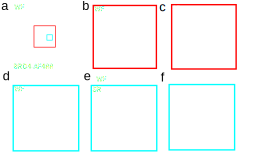
\includegraphics[width=10cm]{Figure_2}
\caption{Energy eigenkets in the position representation for $n=0,10,50$}
\label{fig:method}
\end{figure}

\vspace{0.1in}
\noindent \textbf{(G)} Consider the probability density shown in Figure 2 where $n=50$. It is no coincidence that this value of $n$ is exactly half of the number of samples $N=100$. The Nyquist theorem says that to resolve a signal of frequency $f$ we need a sampling rate of at least $2f$. Put another way, the highest frequency we can resolve, given some sampling rate, is half the sampling rate. Half the sampling rate is the folding frequency, which occurs at $n=50$. Beyond the folding frequency, aliasing occurs and beats are observed.


\vspace{0.1in}
\noindent \textbf{(H)} The unitary transformation that transforms $\hat{H_{0}}$ to the $\ket{\phi_{n}}$ basis is simply

\begin{align*}
\hat{H}_{0}' = U_{0} H_{0} U_{0}^{-1} = T^{-1} H_{0} T
\end{align*}

$\hat{H}_{0}'$ is shown in Figure 3a, and is diagonal.

\vspace{0.1in}
\noindent \textbf{(I)} The values along the diagonal of $\hat{H}_{0}'$ are the energy eigenvalues

\vspace{0.1in}
\noindent \textbf{(J)} The energy eigenvalues are shown in Figure 3b

\vspace{0.1in}
\noindent \textbf{(K)} The energy eigenvalues are the same as they were before the change of basis. All we have done is changed our representation, so they should be. 

\vspace{0.1in}
\noindent \textbf{(L)} Three representative probability distributions are shown in Figure 3d. These are delta functions because we have changed to the energy basis.

\begin{figure}[t!]
\centering
\includegraphics[width=15cm]{Figure_3}
\caption{(A) The Hamiltonian $\hat{H}_{0}'$ after unitary transformation with $U_{0}=T^{-1}$ (B) Eigenvalue spectrum sorted in ascending order (C) Eigenvectors as columns of a matrix (sorted by ascending eigenvalue) (D) Probability densities for a few eigenvectors in the energy basis}
\label{fig:method}
\end{figure}

\section{Part 2}

\vspace{0.1in}
\noindent \textbf{(M)} The Hamiltonian matrix is shown in Figure 4a.

\vspace{0.1in}
\noindent \textbf{(N)} $\hat{H}$ differs from $\hat{H}_{0}$ from zero to the 29th element and the 69th element to the 100th element along the diagonal. This is because we have set $V=V_{L}$ for $0 \leq x \leq 29a$ and $V=V_{R}$ for $69a\leq x \leq 100$. The matrix $\hat{H}$ is shown in Figure 4a, its sorted eigenvectors are shown in Figure 4b, and their corresponding eigenvalues, sorted in ascending order, are shown in Figure 4d. 

\begin{figure}[t!]
\centering
\includegraphics[width=15cm]{Figure_4}
\caption{(A) The Hamiltonian $H$ (B) Eigenvalue spectrum sorted in ascending order (C) Eigenvectors as columns of a matrix (sorted by ascending eigenvalue)}
\label{fig:method}
\end{figure}

\vspace{0.1in}
\noindent \textbf{(O)} The energy eigenvalues for this Hamiltonian are shown in Figure 4d.

\vspace{0.1in}
\noindent \textbf{(P)} Probability distributions for $n=1, 25, 26, 35, 39, 41, 55$ are shown in Figure 5.

\vspace{0.1in}
\noindent \textbf{(Q)} For $n=0$ a particle is most likely to be in the region where $V=0$, which makes sense because this is the ground state. As we increase the energy for $n=24,25,34$, we see that the particle is no longer bound to the potential well ($E > V_{L}$), but it doesn't have enough energy to be found from $69a\leq x \leq 100$ where $V=V_{R}$ ($E < V_{R}$). So we see decaying exponentials there. Furthermore, for $n=38,40,54,55$ we see sinusoidal solutions in both regions $0 \leq x \leq 29a$ and $69a\leq x \leq 100$. Clearly the energy is then high enough for the particle to be found there ($E > V_{R}$).

\vspace{0.1in}
\noindent \textbf{(R)} There are kinks in the energy eigenvalue plot because the nonzero potential modifies the Hilbert space with respect to the free particle Hilbert space. So we shouldn't expect a smoothly varying function.

\vspace{0.1in}
\noindent \textbf{(S)} The matrix after unitary transformation is shown in Figure 6a.

\vspace{0.1in}
\noindent \textbf{(T)} Before we changed basis, we had an eigenvalue equation for $H$. That means that after the change, if we hit certain superpositions of energy eigenkets of $H_0$ with this matrix, we satisfy the eigenvalue equation. So the matrix elements represent the components of that superposition that will satisfy the eigenvalue equation.

\begin{figure}[t!]
\centering
\includegraphics[width=17cm]{Figure_5}
\caption{Probability densities for a few eigenkets of $H$ (see main text for description of the figure)}
\label{fig:method}
\end{figure}
\vspace{0.1in}
\noindent \textbf{(U)} The eigenvalue plot for $U_{0}H U_{0}^{-1}$ is the same as for $H$, as they should be. Again, we have changed our representation but nothing physical has changed.

\vspace{0.1in}
\noindent \textbf{(V)} The probability distributions $|\bra{\phi_{0,m}}\ket{\phi_{n}}|^{2}$ for $n=1, 25, 26, 35, 39, 41, 55$ are shown in Figure 7.

\vspace{0.1in}
\noindent \textbf{(W)} Let $\ket{\phi_{n}}$ be an orthonormal set of energy eigenkets of $\hat{H}$ and $\ket{\phi_{m}}$ be an orthonormal set of eigenkets of $\hat{H_{0}}$. Then $\sum_{m}\ket{\phi_{m}}\bra{\phi_{m}}\ket{\phi_{n}}$ is the representation of $\ket{\phi_{n}}$ in the $\ket{\phi_{m}}$ basis. It follows that $|\bra{\phi_{m}}\ket{\phi_{n}}|^{2}$ is the norm squared of that representation. Ultimately, we see spikes because for certain $m$, because $\bra{\phi_{n}}\ket{\phi_{n}}$ has greater magnitude. One interpretation of this is that we couple together special solutions from the family of solutions to the free particle problem.

\vspace{0.1in}
\noindent \textbf{(X)} The matrix of values $\bra{\phi_{m}}\ket{\phi_{n}}$ is shown in Figure 6c. Each column of this matrix is an eigenvector $\ket{\phi_{n}}$ in the $\ket{\phi_{m}}$ basis. We can see that the kets $\ket{\phi_{n}}$ are superpositions of the plane wave solutions to the free particle problem. This makes sense, because using Fourier analysis, we should be able to construct arbitrary wavefunctions using a basis consisting of fundamental harmonics. Again, by introducing a nonzero potential, we have effectively coupled together special solutions from the family of solutions to the free particle problem.


\begin{figure}[t!]
\centering
\includegraphics[width=16cm]{Figure_6}
\caption{(A) The Hamiltonain after unitary transformation with $U_{0}$ (B) Eigenvalue spectrum sorted in ascending order (C) Eigenvectors as columns of a matrix (sorted by ascending eigenvalue)}
\label{fig:method}
\end{figure}

\begin{figure}[t!]
\centering
\includegraphics[width=17cm]{Figure_7}
\caption{Coupling energy eigenkets by introducing a nonzero potential (see main text for description of the figure)}
\label{fig:method}
\end{figure}
\clearpage
\begin{lstlisting}
import numpy as np
import matplotlib.pyplot as plt
from numpy import linalg as LA

###########################################
# Part 1
###########################################

###########################################
# Define the Hamiltonian H0
###########################################

N = 100 #Number of samples
V = np.zeros((N,)) #Potential
H0 = np.zeros((N,N)) #Hamiltonian matrix H0
H0 += np.diag(2 + V,k=0) #main diagonal
H0 += np.diag(-1*np.ones((N-1,)),k=1) #upper diagonal
H0 += np.diag(-1*np.ones((N-1,)),k=-1) #lower diagonal

###########################################
# Find eigenvectors and eigenvalues of H0
###########################################

vals, vecs = LA.eig(H0)
idx = np.argsort(vals)
vecs = vecs[:,idx]
vals = vals[idx]

###########################################
# Show H0
###########################################

fig, ax = plt.subplots(2,2) #Figure 1
x = ax[0,0].imshow(H0,cmap='coolwarm')
axin1 = ax[0,0].inset_axes([0.575, 0.575, 0.4, 0.4])
y = axin1.imshow(H0[:10,:10],cmap='coolwarm')
plt.colorbar(x,ax=ax[0,0])

###########################################
# Show eigenvectors form an orthonormal set
###########################################

x = ax[0,1].imshow(vecs.T, cmap='coolwarm')
plt.colorbar(x,ax=ax[0,1])
ax[0,1].set_title(r'$T$')
X = vecs.T @ vecs
x = ax[1,0].imshow(X, cmap='coolwarm')
axin1 = ax[1,0].inset_axes([0.575, 0.575, 0.4, 0.4])
y = axin1.imshow(X[:10,:10],cmap='coolwarm')
plt.colorbar(x,ax=ax[1,0])
ax[1,0].set_title(r'$T^{T}T$')

###########################################
# Plot the eigenvalues as a function of n
###########################################


ax[1,1].plot(vals, color='blue')
ax[1,1].set_xlabel('n')
ax[1,1].set_ylabel(r'$\epsilon_{n}$',fontsize=14)
plt.tight_layout()
ax[0,0].text(-0.1, 1.1, 'A', transform=ax[0,0].transAxes, 
            size=10, weight='bold')
ax[0,1].text(-0.1, 1.1, 'B', transform=ax[0,1].transAxes, 
            size=10, weight='bold')
ax[1,0].text(-0.1, 1.1, 'C', transform=ax[1,0].transAxes, 
            size=10, weight='bold')
ax[1,1].text(-0.1, 1.1, 'D', transform=ax[1,1].transAxes, 
            size=10, weight='bold')
plt.show()

###########################################
# Plot a few representative prob dists
###########################################

fig, ax = plt.subplots() #Figure 2
pdf1 = vecs[:,0]**2
pdf2 = vecs[:,10]**2
pdf3 = vecs[:,50]**2

ax.plot(pdf1, color='red',label='n=0')
ax.plot(pdf2, color='blue',label='n=10')
ax.plot(pdf3, color='purple',label='n=50')
ax.set_xlabel('x')
ax.set_ylabel(r'$|\phi_{n}|^{2}$',fontsize=14)
ax.legend(loc='upper right')
plt.show()

###########################################
# Find projection operator to energy basis
###########################################

U0 = LA.inv(vecs)

###########################################
# Diagonalize H0
###########################################

Hd = U0 @ H0 @ LA.inv(U0)

fig, ax = plt.subplots(2,2) #Figure 3
x = ax[0,0].imshow(Hd,cmap='coolwarm')
axin1 = ax[0,0].inset_axes([0.575, 0.575, 0.4, 0.4])
y = axin1.imshow(Hd[:10,:10],cmap='coolwarm')
plt.colorbar(x,ax=ax[0,0])


###########################################
# Find eigenvectors and eigenvalues of H
###########################################

dvals, dvecs = LA.eig(Hd)
idx = np.argsort(dvals)
dvecs = dvecs[:,idx]
dvals = dvals[idx]

###########################################
# Plot the eigenvalues as a function of n
###########################################

x = ax[1,0].imshow(dvecs,cmap='coolwarm')
ax[0,1].plot(dvals, color='blue')
ax[0,1].set_xlabel('n')
ax[0,1].set_ylabel(r'$\epsilon_{n}$',fontsize=14)
plt.colorbar(x,ax=ax[1,0])


###########################################
# Plot a few representative prob dists
###########################################

pdf1 = dvecs[:,10]**2
pdf2 = dvecs[:,20]**2
pdf3 = dvecs[:,50]**2

ax[1,1].plot(pdf1, color='red',label='n=10')
ax[1,1].plot(pdf2, color='blue',label='n=20')
ax[1,1].plot(pdf3, color='purple',label='n=50')
ax[1,1].set_xlabel('n')
ax[1,1].set_ylabel(r'$|\phi_{n}|^{2}$',fontsize=14)
ax[1,1].legend()
ax[0,0].text(-0.1, 1.1, 'A', transform=ax[0,0].transAxes, 
            size=10, weight='bold')
ax[0,1].text(-0.1, 1.1, 'B', transform=ax[0,1].transAxes, 
            size=10, weight='bold')
ax[1,0].text(-0.1, 1.1, 'C', transform=ax[1,0].transAxes, 
            size=10, weight='bold')
ax[1,1].text(-0.1, 1.1, 'D', transform=ax[1,1].transAxes, 
            size=10, weight='bold')
plt.show()

###########################################
# Part 2
###########################################

###########################################
# Define the Hamiltonian H
###########################################

N = 100
Vl = 2
Vr = 3
t = 1
V = np.zeros((N,))
V[:30] = Vl; V[70:] = Vr
H = np.zeros((N,N))
H += np.diag(2*t + V,k=0) #main diagonal
H += np.diag(-t*np.ones((N-1,)),k=1) #upper diagonal
H += np.diag(-t*np.ones((N-1,)),k=-1) #lower diagonal


###########################################
# Find eigenvectors and eigenvalues of H
###########################################

vals, vecs = LA.eig(H)
idx = np.argsort(vals)
vecs = vecs[:,idx]
vals = vals[idx]

###########################################
# Show the Hamiltonian matrix
###########################################

fig, ax = plt.subplots(2,2) #Figure 4
x = ax[0,0].imshow(H,cmap='coolwarm')
axin1 = ax[0,0].inset_axes([0.575, 0.575, 0.4, 0.4])
y = axin1.imshow(H[:10,:10],cmap='coolwarm')
plt.colorbar(x,ax=ax[0,0])


###########################################
# Show eigenvectors form an orthonormal set
###########################################

x = ax[0,1].imshow(vecs.T, cmap='coolwarm')
plt.colorbar(x,ax=ax[0,1])
ax[0,1].set_title(r'$T$')
X = vecs.T @ vecs
x = ax[1,0].imshow(X, cmap='coolwarm')
axin1 = ax[1,0].inset_axes([0.575, 0.575, 0.4, 0.4])
y = axin1.imshow(X[:10,:10],cmap='coolwarm')
plt.colorbar(x,ax=ax[1,0])
ax[1,0].set_title(r'$T^{T}T$')
###########################################
# Plot the eigenvalues as a function of n
###########################################

ax[1,1].plot(vals, color='blue')
ax[1,1].set_xlabel('n')
ax[1,1].set_ylabel(r'$\epsilon_{n}$',fontsize=14)
ax[1,1].set_aspect(15)
ax[0,0].text(-0.1, 1.1, 'A', transform=ax[0,0].transAxes, 
            size=10, weight='bold')
ax[0,1].text(-0.1, 1.1, 'B', transform=ax[0,1].transAxes, 
            size=10, weight='bold')
ax[1,0].text(-0.1, 1.1, 'C', transform=ax[1,0].transAxes, 
            size=10, weight='bold')
ax[1,1].text(-0.1, 1.1, 'D', transform=ax[1,1].transAxes, 
            size=10, weight='bold')
plt.show()

###########################################
# Plot a few representative prob dists
###########################################

pdf1 = vecs[:,0]**2
pdf2 = vecs[:,24]**2
pdf3 = vecs[:,25]**2
pdf4 = vecs[:,34]**2
pdf5 = vecs[:,38]**2
pdf6 = vecs[:,40]**2
pdf7 = vecs[:,54]**2
pdf8 = vecs[:,55]**2

fig, ax = plt.subplots(4,2,sharex=True,figsize=(12,4)) #Figure 5
ax[0,0].plot(pdf1, color='red',label='m=0')
ax1 = ax[0,0].twinx()
ax1.plot(V,color='black',label='V(x)')
ax[1,0].plot(pdf2, color='blue',label='m=24')
ax1 = ax[1,0].twinx()
ax1.plot(V,color='black',label='V(x)')
ax[2,0].plot(pdf3, color='purple',label='m=25')
ax1 = ax[2,0].twinx()
ax1.plot(V,color='black',label='V(x)')
ax[3,0].plot(pdf4, color='purple',label='m=34')
ax1 = ax[3,0].twinx()
ax1.plot(V,color='black',label='V(x)')
ax[0,1].plot(pdf5, color='purple',label='m=38')
ax1 = ax[0,1].twinx()
ax1.plot(V,color='black',label='V(x)')
ax[1,1].plot(pdf6, color='purple',label='m=40')
ax1 = ax[1,1].twinx()
ax1.plot(V,color='black',label='V(x)')
ax[2,1].plot(pdf7, color='purple',label='m=54')
ax1 = ax[2,1].twinx()
ax1.plot(V,color='black',label='V(x)')
ax[3,1].plot(pdf8, color='purple',label='m=55')
ax1 = ax[3,1].twinx()
ax1.plot(V,color='black',label='V(x)')
ax[0,1].set_xlabel('n')
ax[1,1].set_xlabel('n')
ax[2,1].set_xlabel('n')
ax[3,1].set_xlabel('n')
ax[0,0].set_ylabel(r'$|\phi_{0}|^{2}$',fontsize=14)
ax[0,1].set_ylabel(r'$|\phi_{38}|^{2}$',fontsize=14)
ax[1,0].set_ylabel(r'$|\phi_{24}|^{2}$',fontsize=14)
ax[1,1].set_ylabel(r'$|\phi_{40}|^{2}$',fontsize=14)
ax[2,0].set_ylabel(r'$|\phi_{25}|^{2}$',fontsize=14)
ax[2,1].set_ylabel(r'$|\phi_{54}|^{2}$',fontsize=14)
ax[3,0].set_ylabel(r'$|\phi_{34}|^{2}$',fontsize=14)
ax[3,1].set_ylabel(r'$|\phi_{55}|^{2}$',fontsize=14)

plt.tight_layout()
plt.show()


###########################################
# Apply U0 to H
###########################################

H_ = U0 @ H @ LA.inv(U0)

###########################################
# Show the result
###########################################

fig, ax = plt.subplots(1,3) #Figure 6
x = ax[0].imshow(H_,cmap='coolwarm')
axin1 = ax[0].inset_axes([0.575, 0.575, 0.4, 0.4])
y = axin1.imshow(H_[:10,:10],cmap='coolwarm')
plt.colorbar(x,ax=ax[0])


###########################################
# Find eigenvectors and eigenvalues of H
###########################################

vals, vecs = LA.eig(H_)
idx = np.argsort(vals)
vecs = vecs[:,idx]
vals = vals[idx]

###########################################
# Plot the eigenvalues as a function of n
###########################################

ax[1].plot(vals, color='blue')
ax[1].set_xlabel('n')
ax[1].set_ylabel(r'$\epsilon_{n}$',fontsize=14)
ax[2].imshow(vecs,cmap='coolwarm')
ax[0].text(-0.1, 1.1, 'A', transform=ax[0].transAxes, 
            size=10, weight='bold')
ax[1].text(-0.1, 1.1, 'B', transform=ax[1].transAxes, 
            size=10, weight='bold')
ax[2].text(-0.1, 1.1, 'C', transform=ax[2].transAxes, 
            size=10, weight='bold')
plt.show()

###########################################
# Plot a few representative prob dists
###########################################

pdf1 = vecs[:,0]**2
pdf2 = vecs[:,24]**2
pdf3 = vecs[:,25]**2
pdf4 = vecs[:,34]**2
pdf5 = vecs[:,38]**2
pdf6 = vecs[:,40]**2
pdf7 = vecs[:,54]**2
pdf8 = vecs[:,55]**2

fig, ax = plt.subplots(4,2,sharex=True,figsize=(12,4)) #Figure 7
ax[0,0].plot(pdf1, color='red',label='m=0')
ax[1,0].plot(pdf2, color='blue',label='m=24')
ax[2,0].plot(pdf3, color='purple',label='m=25')
ax[3,0].plot(pdf4, color='purple',label='m=34')
ax[0,1].plot(pdf5, color='purple',label='m=38')
ax[1,1].plot(pdf6, color='purple',label='m=40')
ax[2,1].plot(pdf7, color='purple',label='m=54')
ax[3,1].plot(pdf8, color='purple',label='m=55')
ax[0,1].set_xlabel('n')
ax[1,1].set_xlabel('n')
ax[2,1].set_xlabel('n')
ax[3,1].set_xlabel('n')
ax[0,0].set_ylabel(r'$|\phi_{m}^{*}\phi_{0}|^{2}$',fontsize=14)
ax[0,1].set_ylabel(r'$|\phi_{m}^{*}\phi_{38}|^{2}$',fontsize=14)
ax[1,0].set_ylabel(r'$|\phi_{m}^{*}\phi_{24}|^{2}$',fontsize=14)
ax[1,1].set_ylabel(r'$|\phi_{m}^{*}\phi_{40}|^{2}$',fontsize=14)
ax[2,0].set_ylabel(r'$|\phi_{m}^{*}\phi_{25}|^{2}$',fontsize=14)
ax[2,1].set_ylabel(r'$|\phi_{m}^{*}\phi_{54}|^{2}$',fontsize=14)
ax[3,0].set_ylabel(r'$|\phi_{m}^{*}\phi_{34}|^{2}$',fontsize=14)
ax[3,1].set_ylabel(r'$|\phi_{m}^{*}\phi_{55}|^{2}$',fontsize=14)


plt.tight_layout()
plt.show()




\end{lstlisting}

\end{document}